\documentclass[]{scrartcl}

\usepackage{mathtools}
\usepackage{subfigure}
\renewcommand{\familydefault}{\sfdefault}
\usepackage{color}
\usepackage{listings}
\definecolor{pblue}{rgb}{0.13,0.13,1}
\definecolor{pgreen}{rgb}{0,0.5,0}
\definecolor{pred}{rgb}{0.9,0,0}
\definecolor{pgrey}{rgb}{0.46,0.45,0.48}
\setlength{\parindent}{0pt}

\lstset{language=Java,
	showspaces=false,
	showtabs=false,
	breaklines=true,
	showstringspaces=false,
	breakatwhitespace=true,
	commentstyle=\color{pgreen},
	keywordstyle=\color{pblue},
	stringstyle=\color{pred},
	basicstyle=\footnotesize
}

%opening
\title{Intelligent Data Management - Exercise 3}
\author{Christoph Prinz}

\begin{document}

\maketitle

\subsection*{Assignment 1}

a) Minhash Signature:\\

\begin{tabular}{c|c|c|c|c||c|c|c}
	Element & $S_1$ & $S_2$ & $S_3$  & $S_4$ & $h_1$ & $h_2$ & $h_3$  \\ 
	\hline\hline
	0 & 0 & 1 & 0 & 1 & 1  & 2 & 2 \\ 
	\hline 
	1 & 0 & 1 & 0 & 0 & 3 & 5  & 1 \\ 
	\hline 
	2 & 1 & 0 & 0 & 1 & 5 & 2 & 0  \\ 
	\hline 
	3 & 0 & 0 & 1 & 0 & 1 & 5 & 5 \\ 
	\hline 
	4 & 0 & 0 & 1 & 1 & 3 & 2 & 4 \\ 
	\hline 
	5 & 1 & 0 & 0 & 0 & 5 & 5 & 3 \\ 
\end{tabular}


\vspace{1cm}

b) Only $h_3$ provides a sufficient hash-function because it offers different hashed for every element. 

\vspace{1cm}

Minhash-Signature Step 1:\\
\begin{tabular}{c||c|c|c|c}
	& $S_1$ & $S_2$ & $S_3$ &$S_4$  \\ 
	\hline \hline
 $h_1$	& $\infty$ & $\infty$ & $\infty$ & $\infty$ \\ 
	\hline 
$h_2$	& $\infty$ & $\infty$ & $\infty$ & $\infty$ \\ 
	\hline 
$h_3$	& $\infty$ & $\infty$ & $\infty$ & $\infty$ \\ 
\end{tabular}

\vspace{1cm}

Minhash-Signature Step 2:\\
\begin{tabular}{c||c|c|c|c}
			& $S_1$ & $S_2$ & $S_3$ &$S_4$  \\ 
	\hline \hline
	$h_1$	&  $\infty$ & 1 & $\infty$ & 1 \\ 
	\hline 
	$h_2$	&  $\infty$ & 2 & $\infty$ & 2 \\ 
	\hline 
	$h_3$	&  $\infty$ & 2 & $\infty$ & 2 \\ 
\end{tabular} 

\vspace{1cm}

Minhash-Signature Step 3:\\
\begin{tabular}{c||c|c|c|c}
	& $S_1$ & $S_2$ & $S_3$ &$S_4$  \\ 
	\hline \hline
	$h_1$	&  $\infty$ & 1 & $\infty$ & 1 \\ 
	\hline 
	$h_2$	&  $\infty$ & 2 & $\infty$ & 2 \\ 
	\hline 
	$h_3$	&  $\infty$ & 1 & $\infty$ & 2 \\ 
\end{tabular} 

\vspace{1cm}

Minhash-Signature Step 4:\\
\begin{tabular}{c||c|c|c|c}
			& $S_1$ & $S_2$ & $S_3$ &$S_4$  \\ 
	\hline \hline
	$h_1$	&  5 & 1 & $\infty$ & 1 \\ 
	\hline 
	$h_2$	&  2 & 2 & $\infty$ & 2 \\ 
	\hline 
	$h_3$	&  0 & 1 & $\infty$ & 0 \\ 
\end{tabular} 

\vspace{1cm}

Minhash-Signature Step 5:\\
\begin{tabular}{c||c|c|c|c}
	& $S_1$ & $S_2$ & $S_3$ &$S_4$  \\ 
	\hline \hline
	$h_1$	&  5 & 1 & 1 & 1 \\ 
	\hline 
	$h_2$	&  2 & 2 & 2 & 2 \\ 
	\hline 
	$h_3$	&  0 & 1 & 4 & 0 \\ 
\end{tabular} 

\vspace{1cm}

Final Minhash-Signature (After Step 6):\\
\begin{tabular}{c||c|c|c|c}
	& $S_1$ & $S_2$ & $S_3$ &$S_4$  \\ 
	\hline \hline
	$h_1$	&  5 & 1 & 1 & 1 \\ 
	\hline 
	$h_2$	&  2 & 2 & 2 & 2 \\ 
	\hline 
	$h_3$	&  0 & 1 & 4 & 0 \\ 
\end{tabular} 

\vspace{1cm}

Jaccard Similarities formula = $|S \cap T| \div |S \cup T|$ \\

$SIM(S_1, S_2) = SIM(\{2, 5\}, \{0, 1\}) = 0$\\\\
$SIM(S_1, S_3) = SIM(\{2, 5\},\{3, 4\}) = 0$\\\\
$SIM(S_1, S_4) = SIM(\{2, 5\}, \{0, 2, 4\}) = \frac{1}{4}$\\\\
$SIM(S_2, S_3) = SIM(\{0, 1\}, \{3, 4\}) = 0$\\\\
$SIM(S_2, S_4) = SIM(\{0, 1\}, \{0, 2, 4\}) = \frac{1}{4}$\\\\
$SIM(S_3, S_4) = SIM(\{3, 4\}, \{0, 2, 4\}) = \frac{1}{4}$\\\\

\subsection*{Assignment 2}

Plots for s-curve:

\begin{figure}[h!]
	\centering
	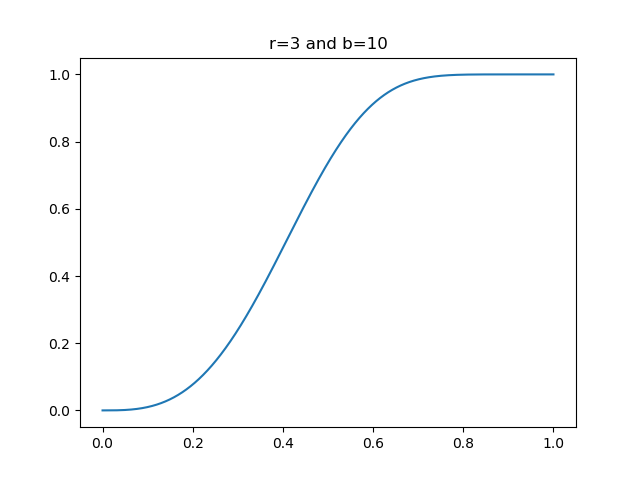
\includegraphics[width=0.5\linewidth]{Exercise4_plots/plot_1}
\end{figure}

\begin{figure}[h!]
	\centering
	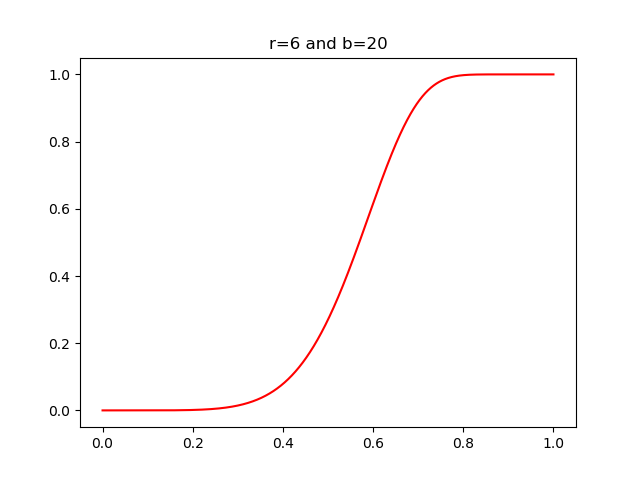
\includegraphics[width=0.5\linewidth]{Exercise4_plots/plot_2}
\end{figure}

\begin{figure}[h!]
	\centering
	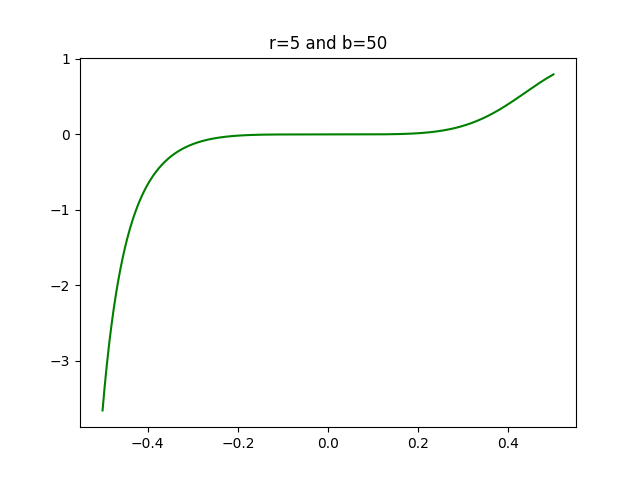
\includegraphics[width=0.5\linewidth]{Exercise4_plots/plot_3}
\end{figure}

\vspace{5cm}
s that fulfils $1-(1-s^r)^b = \frac{1}{2}$:\\

a) $ s_1 = \sqrt[3]{1-\frac{1}{\sqrt[10]{2}}} \approx 0.406 $\\
$ s_2 = \sqrt[3]{1+\frac{1}{\sqrt[10]{2}}} \approx 1.246 $\\
$1/b^{1/r} \approx 0.464$\\\\

b) $ s_1 = \sqrt[6]{1-\frac{1}{\sqrt[20]{2}}} \approx 0.569 $\\
$ s_2 = \sqrt[6]{1+\frac{1}{\sqrt[20]{2}}} \approx 1.194 $\\
$1/b^{1/r}\approx 0.607$\\\\

c) $ s_1 = \sqrt[5]{1-\frac{1}{\sqrt[50]{2}}} \approx 0.424 $\\
$ s_2 = \sqrt[5]{1+\frac{1}{\sqrt[50]{2}}} \approx 1.147 $\\
$1/b^{1/r} \approx 0.457$\\\\

\end{document}
